\section*{SSB 9.3}
At end of document

\section*{Problem 2}
\subsection*{Part a}
The dispersion relation is
\eq{
\omega(k) &= 2\sqrt{\frac{\kappa}{m}}|\sin(\frac{\kappa a}{2})|\\
\frac{\omega^2}{4}\frac{m}{\kappa} &= \sin^2(\frac{k a}{2})\\
k &= \frac{2}{a}\arcsin(\frac{\omega}{2}\sqrt{\frac{m}{\kappa}})\\
k &\equiv \frac{2}{a}\arcsin(\omega')
}
Where we have taken the principal branch due to the absolute value. The vibrational modes ($\nu$ or $N$) go as
\eq{
\nu(k) &= \frac{a}{2\pi}\int dk = \frac{a}{\pi}k\\
&=  \frac{2}{\pi}\arcsin(\omega')
}
The density of states is then
\eq{
g(\omega) &= \frac{d\nu}{d\omega} = \frac{\partial \nu}{\partial \omega'}\frac{d\omega'}{d\omega}\\
&= \frac{1}{\pi}\sqrt{\frac{m}{\kappa}} \frac{1}{\sqrt{1-\omega'^2}}\\
g'(\omega') &\equiv \frac{1}{\pi}\frac{1}{\sqrt{1-\omega'^2}}
}
Where $\omega'$ is in units of $\sqrt{\frac{m}{\kappa}}$ and the density of the states is in units of $\sqrt{\frac{\kappa}{m}}$.
\subsection*{Part b}
\begin{figure}[h]
    \centering
    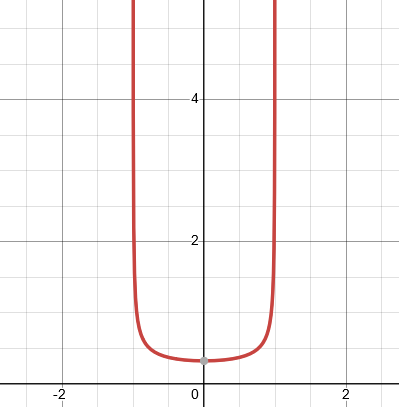
\includegraphics[width=1\linewidth]{Resources//140A//Homework 4/Screenshot 2024-11-10 195146.png}
    \label{fig:enter-label}
\end{figure}


\subsection*{Part c}
The energy per mode goes as
\eq{
\frac{C}{N} &= \frac{a}{2\pi}\partial_T \int_{-\frac{\pi}{a}}^{\frac{\pi}{a}} \hbar \omega(k)(n_B+\frac{1}{2})dk\\
&= \frac{a}{2\pi}\int_{-\frac{\pi}{a}}^{\frac{\pi}{a}} \hbar \omega(k) \partial_T(\frac{1}{\exp(\frac{\hbar \omega(k)}{k_BT})-1}) dk\\
&\approx \frac{a}{2\pi}\int_{-\frac{\pi}{a}}^{\frac{\pi}{a}} \hbar \omega(k) \partial_T \frac{k_BT}{\hbar \omega(k)}dk\\
&\approx \frac{a}{2\pi}k_B\int_{-\frac{\pi}{a}}^{\frac{\pi}{a}}dk\\
&\approx \frac{a}{2\pi}k_B\frac{2\pi}{a}\\
&\approx k_B
}

\section*{SSB 10.1}
At end of document

\section*{Problem 4}
\subsection*{Part a}
The total size of the Brillouin zone is
\eq{
4a \rightarrow \frac{2\pi}{4a} = \frac{\pi}{2a}
}
With maximum and minimum $k$ vectors, respectively,
\eq{
k_\pm &= \pm \frac{\pi}{4a}
}
Rest at end of document

\section*{Problem 5}
\subsection*{Part a}
Copper has one atom per unit cell, with 3 translational degrees of freedom, which correspond to acoustic branches.

Diamond has two atoms per unit cell, with 3 translational degrees of freedom, which correspond to acoustic and optical branches since we can now have out of phase oscillations.

\subsection*{Part b}
The highest occupied linear frequency for Cu is
\eq{
f_{max} &= 7\textrm{ THz}\\
\implies \omega_{max} &\approx 44 \textrm{ THz}\\
\implies \theta_D = \frac{\hbar}{k_B} \omega_{max} &\approx 336 \textrm{ K}
}
The highest occupied linear frequency for Diamond is
\eq{
f_{max} &= 44\textrm{ THz}\\
\implies \omega_{max} &\approx 276.46 \textrm{ THz}\\
\implies \theta_D = \frac{\hbar}{k_B} \omega_{max} &\approx 2111 \textrm{ K}
}
\subsection*{Part c}
We can estimate the dispersion relation to first order. Assuming $\Gamma \chi$ is the length in reciprocal space
\eq{
v &= \frac{\omega}{k} = 2\pi\frac{f}{k}\\
&\approx 5 \textrm{ THz}\cdot 362 \textrm{ pm}\\
&\approx 1.8 \frac{\textrm{ km}}{\textrm{s}}
}